\documentclass[a4paper,14pt]{article}

\usepackage{fvextra}
\usepackage{verbatim}

\DefineVerbatimEnvironment{Verbatim}{Verbatim}{breaklines=true}



\usepackage{eso-pic}


\usepackage{float}
\usepackage{graphicx}

\usepackage{listings}
\usepackage{xcolor}

\usepackage[utf8]{inputenc}
\usepackage[english, russian]{babel}


\setlength{\parindent}{12.5mm} 



\lstset{
    basicstyle=\ttfamily\small, % Шрифт и размер
    breaklines=true,             % Перенос строк
    breakatwhitespace=false,     % Перенос по пробелам
    columns=flexible,            % Гибкий размер колонок
%     frame=single,                % Рамка вокруг кода
%     backgroundcolor=\color{lightgray!20}, % Цвет фона
}


\usepackage{calc}
\usepackage{background}


\usepackage[height=297mm, width=210mm, left=3cm, top=2cm, right=1cm, bottom=2cm]{geometry}


\newcommand{\chipher}{
        {\fontsize{16pt}{16pt}\selectfont  КР.ИИ-21.210574-3 81 00}
}




\begin{document}
        \sloppy
        
        \pagestyle{empty}
        \fontsize{14}{17.5}\selectfont    


        


\newcommand{\applicationTitlePage}{

    \begin{center}
        МИНИСТЕРСТВО ОБРАЗОВАНИЯ РЕСПУБЛИКИ БЕЛАРУСЬ \\
        УЧРЕЖДЕНИЕ ОБРАЗОВАНИЯ \\
        <<БРЕСТСКИЙ ГОСУДАРСТВЕННЫЙ ТЕХНИЧЕСКИЙ УНИВЕРСИТЕТ>> \\
        ФАКУЛЬТЕТ ЭЛЕКТРОННО-ИНФОРМАЦИОННЫХ СИСТЕМ \\
        Кафедра интеллектуальных информационных технологий \\[4cm]
        
         
            \MakeUppercase{
                {\bf Приложение А \\}
                
            }
            <<Текст программы>> \\[4cm]
        
           
            
        

    \end{center}

    \begin{flushright}
        \begin{minipage}{0.35\textwidth}
            \begin{flushleft}
                {\bf Выполнил:} \\
                студент 4-го курса, \\
                ФЭИС, \\
                группы ИИ-21 \\
                Худик А.А. \\
                {\bf Проверил:} \\
                Кулеша В.И.
            \end{flushleft}
        \end{minipage}
    \end{flushright}

    \vfill 

    \begin{center}
        Брест \the\year
    \end{center}

    \newpage

}



        \newcommand{\applicationContent}{
    Схема взаимодействия компонентов системы (рис. 1).
    \begin{figure}[H]
        \centering
        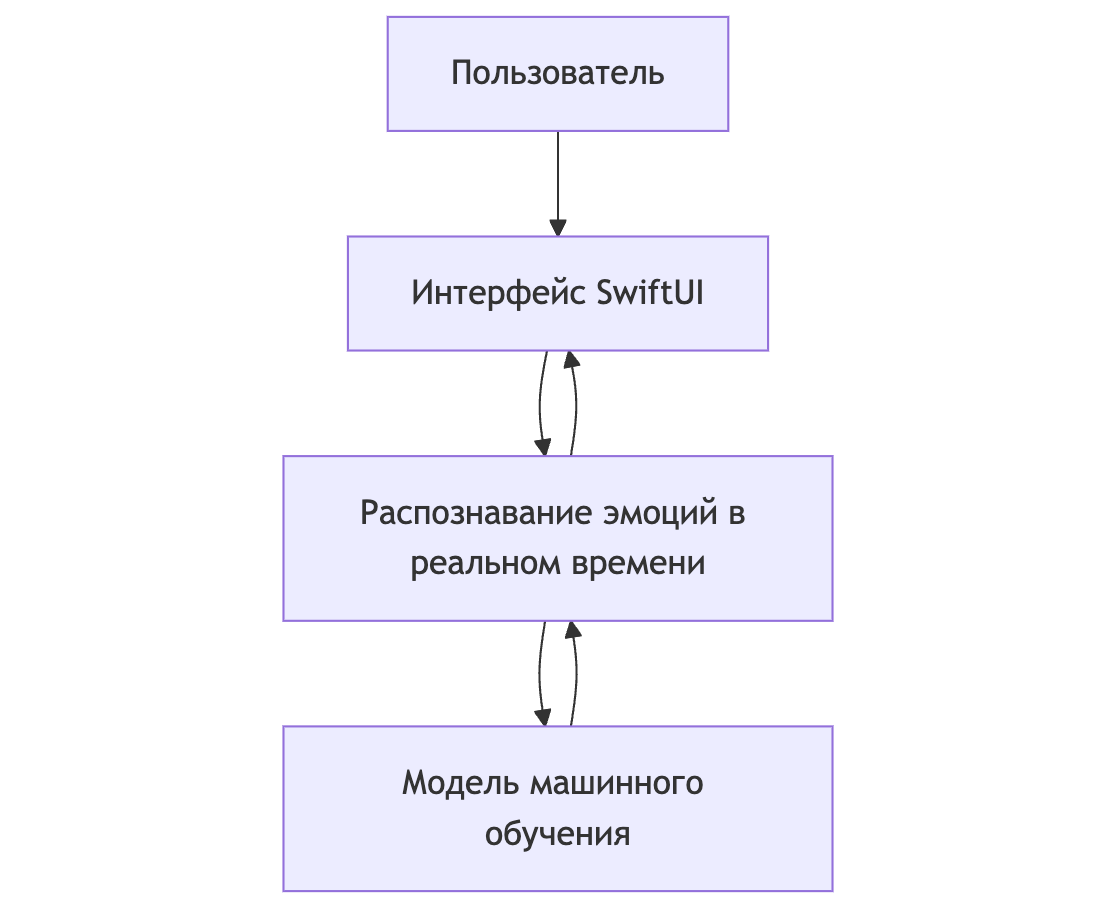
\includegraphics[width=0.8\textwidth]{application/components.png} 
        \caption{Схема взаимодействия компонентов системы}
    \end{figure}

    \newpage
    
    Схема обработки видео (рис. 2).
    \begin{figure}[H]
        \centering
        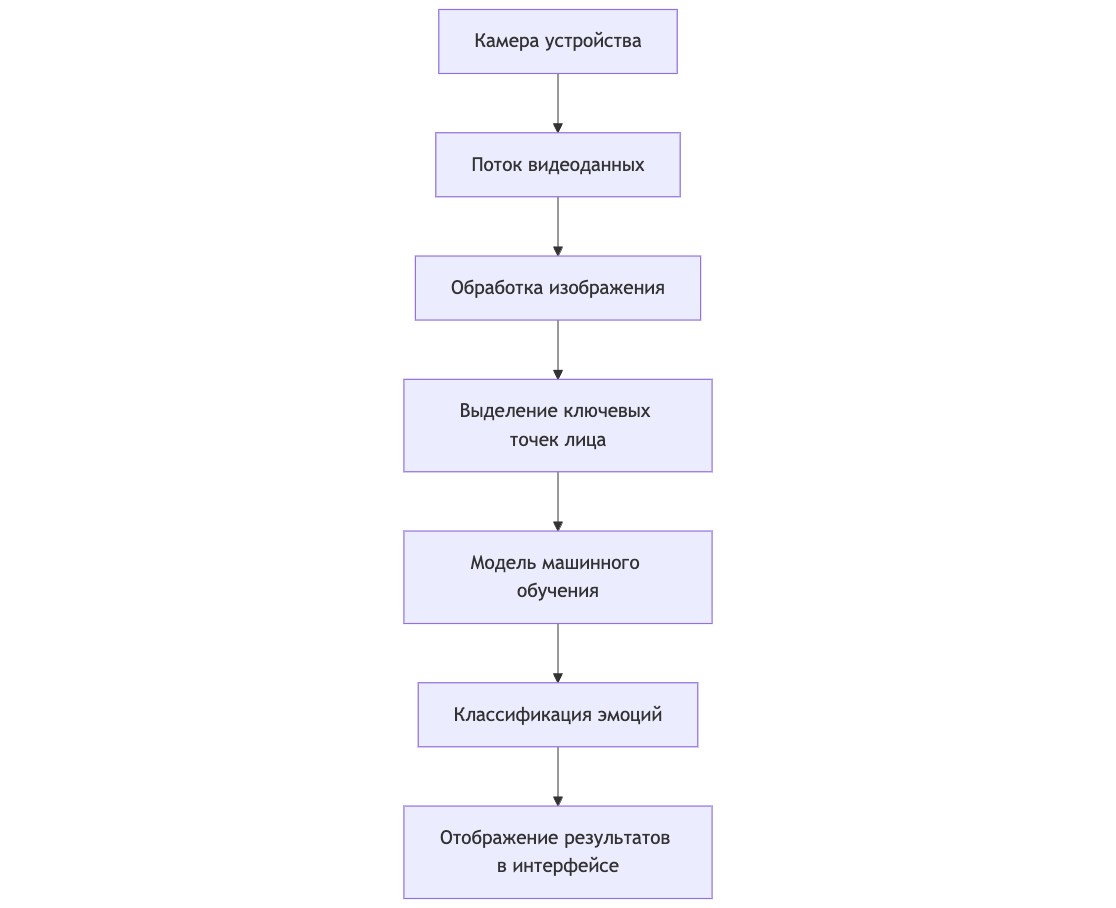
\includegraphics[width=0.8\textwidth]{application/DB-scheme.png} 
        \caption{Схема обработки видео}
    \end{figure}
}

        \NoBgThispage
        \applicationTitlePage

        \backgroundsetup{
                scale=1,
                color=black,
                opacity=1,
                angle=0,
                position=current page.center,
                vshift=0cm, hshift=0cm,
                contents={
\includegraphics[width=\paperwidth,height=\paperheight]{application/border11.png}}
        }

        \applicationContent
    
\end{document}
